\section{Notions avancées}
\label{notion}
Un exemple d'utilisation de l' ADC est la gestion des signaux PWM (Pulse Width Modulation) ou  MLI (Modulation de Largeur d'Impulsions) en français. 
\paragraph{}
Le principe général de la modulation PWM est qu'en appliquant une succession d'états discrets pendant des durées bien définies, on peut générer des signaux continus. La valeur moyenne du signal obtenu est alors égale au rapport cyclique du module PWM:   $\text {rapport cyclique} =  \frac{\text{Temps haut}}{\text{Période}}$ . Un exemple pour une tension d'entrée de 3V vous est présenté à la FIGURE \ref{pwm}.



\begin{figure}[h]
\begin{center}
\begin{framed}
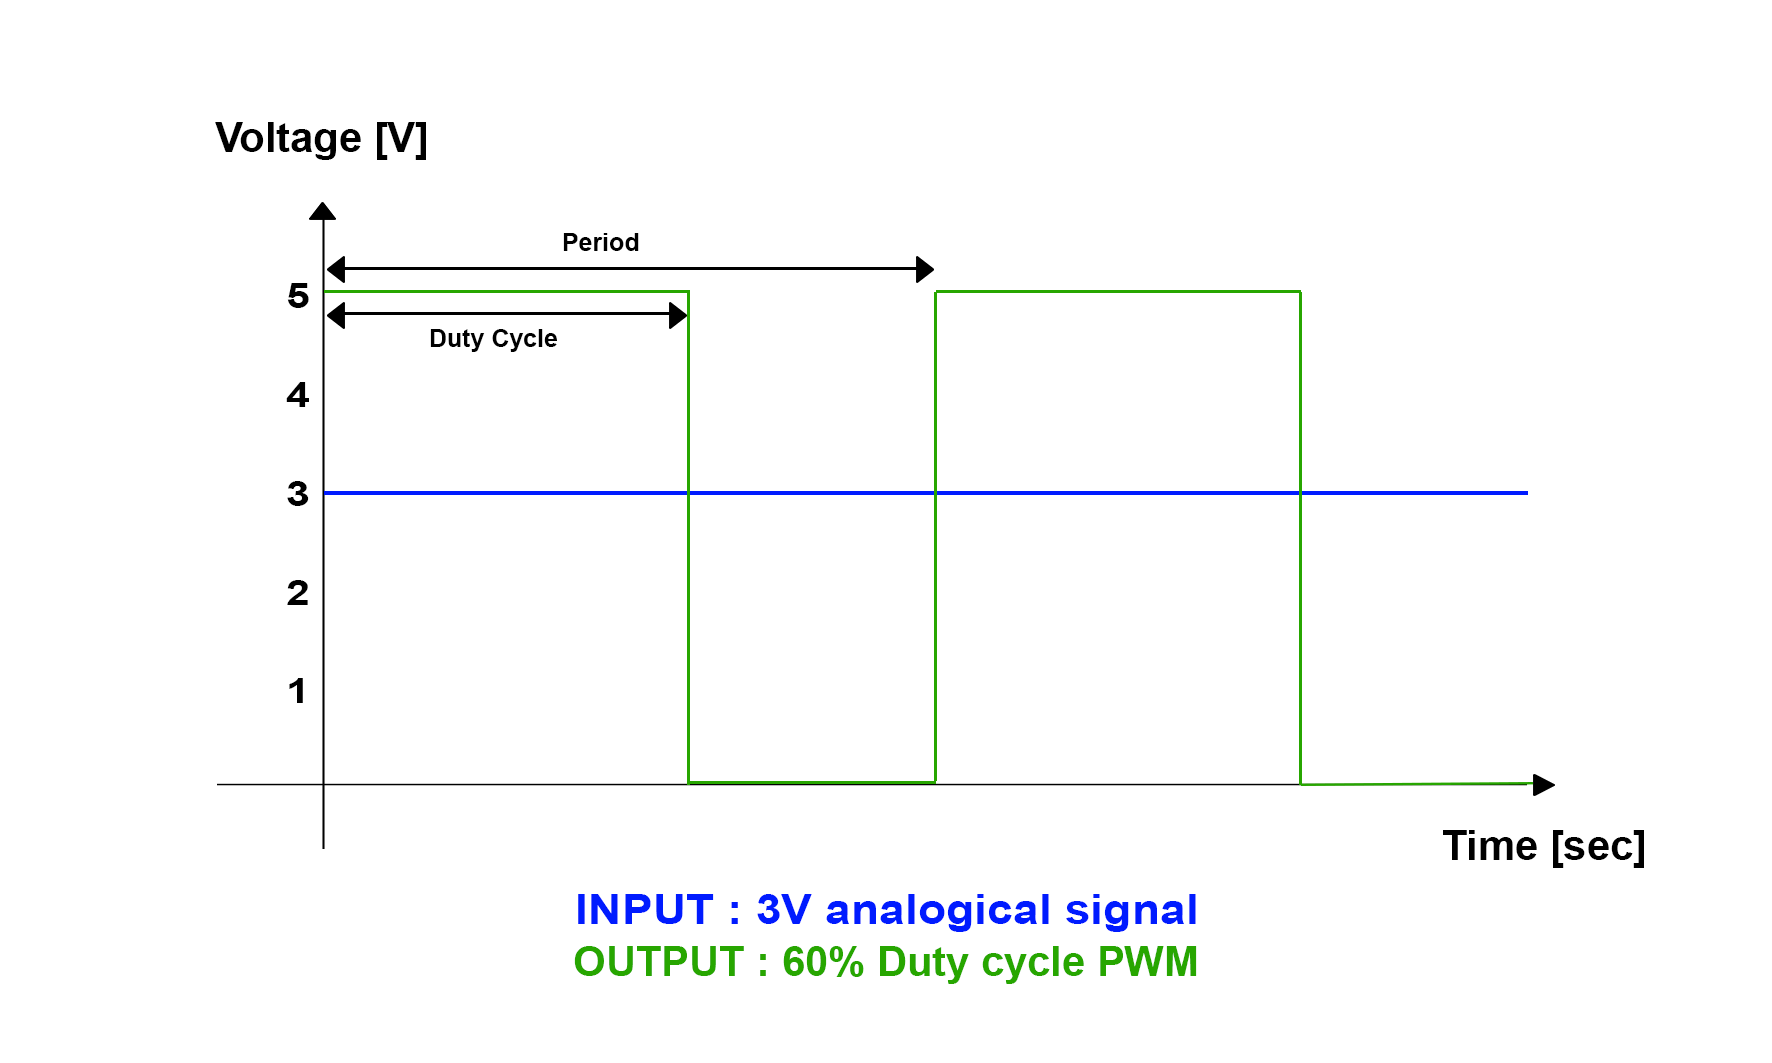
\includegraphics[scale=0.8]{images/pwm.png}
\caption{Transformation d'un signal analogique en signal PWM de tension équivalente}
\label{pwm}
\end{framed}
\end{center}
\end{figure}

\paragraph{}
Une application concrète de ces notions est le contrôle d'un moteur DC au moyen d'un signal PWM. Le moteur est placé dans un montage en pont H dont l'ouverture et la fermeture des interrupeurs est commandée par le signal PWM (voir FIGURE \ref{pontH}). Afin de gérer le sens de rotation du moteur ainsi que sa vitesse, on utilise un potentiomètre et un convertisseur Analogique-Numérique. Celui-ci aura alors pour fonction de traduire la valeur analogique de la tension lue sur le potentiomètre en un rapport cyclique pour le module PWM. Ainsi, par exemple,  si le potentiomètre est mis sur la résistance minimale, l'ADC convertira cette valeur en un rapport cyclique minimum et le moteur sera à basse vitesse\footnote{Nb: nous ne développeront cependant pas le code pour ce genre d'application, car il s'agit d'une utilisation directe d'une PWM, mais indirecte d'un ADC.}.

\begin{figure}[h]
\begin{center}
\begin{framed}
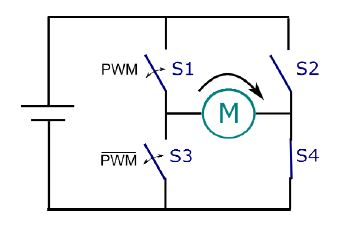
\includegraphics[scale=0.8]{images/pontH.jpg}
\caption{Contrôle d'un moteur DC via un montage en pont H}
\label{pontH}
\end{framed}
\end{center}
\end{figure}

\paragraph{}
Utilisation du signal numérique de sortie de l'ADC pour créer une PWM, via les librairies du compilateur XC8:

\paragraph{Création de la PWM} paramétrage de la période\footnote{
le calcul de la durée de la période de la PWM se fait grâce à la formule $period =[(period ) + 1] x 4 x TOSC x TMR2 prescaler$. Cette valeur sera renseignée comme paramètre de la fonction OpenPMMx() et du mode.}
\begin{lstlisting}
OpenPWM1(0xFF);
SetOutputPWM1(SINGLE_OUT, PWM_MODE_1);
\end{lstlisting}

\paragraph{Conversion} On suppose l'ADC correctement paramétré pour lire la tension sur le potentiomètre (voir Section \ref{programmation}).
Les fonctions \textbf{ConvertADC()}, \textbf{BusyADC()} et \textbf{ReadADC()} permettent respectivement : 
\begin{itemize}
\item de demander à l'ADC de lancer une mesure
\item de vérifier si il a fini de convertir la tension analogique
\item de lire le résultat de la conversion
\end{itemize}

\begin{lstlisting}
ConvertADC();
while(BusyADC());
value = ReadADC();
\end{lstlisting}

\paragraph{Redirection de la sortie numérique de l'ADC vers la PWM}.
\begin{lstlisting}
SetDCPWM1(value);
\end{lstlisting}

\paragraph{Fermeture de l'ADC à la fin du programme}.
\begin{lstlisting}
CloseADC();
\end{lstlisting}

